\chapter{Theoretical Background}
\label{chap:theory_SAXS}
In this chapter, the basic physical principles underlying the operation of small-angle X-ray scattering are presented, focusing principally on the interaction between X-rays and matter and the elastic scattering of X-rays by an ensemble of electrons. The fundamental theoretical background of SAXS is also introduced, jointly with the analytical expressions of the form factors used in this work. An entire section is devoted to the theoretical framework used in contrast variation experiments in SAXS, where concepts such as the isoscattering point and the basic functions approach are introduced.

\section{Interaction of X-rays and matter}

X-rays are electromagnetic waves which propagate in vacuum along the direction of the wavevector $\vect{k}$. The incident X-ray radiation can be described by the wave function of a monochromatic plane wave:

\begin{equation}
        \label{eq:IncidentWave}
        \Psi_0\left( \vect{r} \right)=A_0 e^{i \vect{k}\vect{r} }
\end{equation}

where the wavenumber $k=\abs{\vect{k}}$ is related to the X-ray wavelength $\lambda$ by $k=\sfrac{2\pi}{\lambda}$. Conventionally, X-ray wavelengths range between 0.01 and a few nanometres, although SAXS experiments are conducted normally at the hard X-ray range, e.g. at wavelenghts between 0.02 and 0.8 nm. Due to the wave-particle duality of electromagnetic radiation, X-rays possess a particle nature as well, represented by the quantization of light into an ensemble of photons with an energy $\hbar \omega$. The photon energy is related to the X-ray wavelength by \citep{als-nielsen_elements_2011}

\begin{equation}
        \lambda = \frac{h c}{E_{ph}}
\end{equation}

where $h$ is the Planck's constant and $c$ is the speed of light in vacuum. The photon energies employed typically in SAXS experiments stretch between the silicon K-edge at 1.7 keV and some dozens of keV, including the classic copper K$_{\alpha}$ emission line at 8 keV.

\begin{figure}[hbt]%[htbp]
	\centering
	        \def\svgwidth{0.8\linewidth}
		\input{Figures/BeerLambertScheme.pdf_tex}
		\caption[Depiction of the Beer-Lambert law.]{The Beer-Lambert law is schematically depicted: The attenuation of X-rays through a medium of thickness $d$ and attenuation coefficient $\mu$ behaves accordingly to the expression \ref{eq:BeerLambertLaw}.}
		\label{fig:BeerLambertScheme}
\end{figure}


\subsection{Beer-Lambert law}
\label{sec:BeerLambert}

The interaction of X-ray photons and matter produce an attenuation of the incident radiation intensity $I_0$ which is related to the properties and volume of the material. The decrease of the intensity through a medium is schematically depicted in figure \ref{fig:BeerLambertScheme} and described by the Beer-Lambert law \citep{als-nielsen_elements_2011}:

\begin{equation}
        \label{eq:BeerLambertLaw}
        I\left( x \right)=I_0e^{-\mu x}
\end{equation}

where $\mu$ is the linear attenuation coefficient and $x$ is the radiation path length. The attenuation coefficient is dependent on the material composition and the photon energy and is directly related to the extinction coefficient $\beta$, e.g. the imaginary part of the refraction index $n$, by \citep{marr_handbook_1987}

\begin{equation}
        \mu (E) = \frac{4\pi}{hc} E \beta(E)
\end{equation}

Considering that the refractive index is expressed generally by $n = 1 - \delta +i \beta$ and $\delta<10^{-3}$ in the X-ray regime \citep{henke_x-ray_1993}, refraction effects can be neglected in scattering experiments because $\Re(n)$ is very close but smaller than unity.

When the attenuating medium is composed of different atomic species, $\mu$ can be expressed as the summation of each component attenuation coefficient $\mu_i$:

\begin{equation}
        \label{eq:AttenuationMultiComponent}
        \mu = \sum_i \mu^i = \sum_i \rho_e^i \sigma^i  =N_A\sum_i  \frac{Z^i}{A^i} \rho^i \sigma^i
\end{equation}

where $N_A$ is the Avogadro constant, $\sigma$ is the attenuation cross-section and $\rho_e$ is the number density of absorbing centres. The cross-section $\sigma$ is defined as the effective area in which photon-matter events occur. In the X-ray regime, photons interact principally with the atomic electrons, thus $\rho_e$ is the electron density and is directly proportional to the atomic number $Z$, the atomic mass number $A$ and the mass density $\rho$ of the component $i$. 

In fact, the attenuation cross-section $\sigma$ is dependent upon the several different mechanisms in which a X-ray photon interacts with the atomic electrons. The 3 most relevant effects are the photoelectron absorption, the coherent scattering and the incoherent scattering, which sum up to the total attenuation coefficient:

\begin{equation}
        \mu = \rho_e (\tau_{\text{abs}}+\sigma_{\text{scat, coh}}+\sigma_{\text{scat, incoh}})
\end{equation}

When the X-ray photon is completely absorbed by the atom, the event is called photoelectron absorption because a photoelectron with the excess energy is expelled from an inner atomic shell, leaving the atom ionized. The created core-hole is consequently filled by an electron from an outer shell either by a radiative process, i.e. \emph{fluorescence}, or by a non-radiative mechanism emitting a secondary electron, i.e. \emph{Auger effect}. The photoelectric effect is the predominant contribution to the attenuation cross-section principally at low X-ray energies and the ultraviolet regime, as shown in figure \ref{fig:AttenuationWater}. 

\begin{figure}%[htbp]
	\centering
		% GNUPLOT: LaTeX picture with Postscript
\begingroup
  \makeatletter
  \providecommand\color[2][]{%
    \GenericError{(gnuplot) \space\space\space\@spaces}{%
      Package color not loaded in conjunction with
      terminal option `colourtext'%
    }{See the gnuplot documentation for explanation.%
    }{Either use 'blacktext' in gnuplot or load the package
      color.sty in LaTeX.}%
    \renewcommand\color[2][]{}%
  }%
  \providecommand\includegraphics[2][]{%
    \GenericError{(gnuplot) \space\space\space\@spaces}{%
      Package graphicx or graphics not loaded%
    }{See the gnuplot documentation for explanation.%
    }{The gnuplot epslatex terminal needs graphicx.sty or graphics.sty.}%
    \renewcommand\includegraphics[2][]{}%
  }%
  \providecommand\rotatebox[2]{#2}%
  \@ifundefined{ifGPcolor}{%
    \newif\ifGPcolor
    \GPcolortrue
  }{}%
  \@ifundefined{ifGPblacktext}{%
    \newif\ifGPblacktext
    \GPblacktextfalse
  }{}%
  % define a \g@addto@macro without @ in the name:
  \let\gplgaddtomacro\g@addto@macro
  % define empty templates for all commands taking text:
  \gdef\gplbacktext{}%
  \gdef\gplfronttext{}%
  \makeatother
  \ifGPblacktext
    % no textcolor at all
    \def\colorrgb#1{}%
    \def\colorgray#1{}%
  \else
    % gray or color?
    \ifGPcolor
      \def\colorrgb#1{\color[rgb]{#1}}%
      \def\colorgray#1{\color[gray]{#1}}%
      \expandafter\def\csname LTw\endcsname{\color{white}}%
      \expandafter\def\csname LTb\endcsname{\color{black}}%
      \expandafter\def\csname LTa\endcsname{\color{black}}%
      \expandafter\def\csname LT0\endcsname{\color[rgb]{1,0,0}}%
      \expandafter\def\csname LT1\endcsname{\color[rgb]{0,1,0}}%
      \expandafter\def\csname LT2\endcsname{\color[rgb]{0,0,1}}%
      \expandafter\def\csname LT3\endcsname{\color[rgb]{1,0,1}}%
      \expandafter\def\csname LT4\endcsname{\color[rgb]{0,1,1}}%
      \expandafter\def\csname LT5\endcsname{\color[rgb]{1,1,0}}%
      \expandafter\def\csname LT6\endcsname{\color[rgb]{0,0,0}}%
      \expandafter\def\csname LT7\endcsname{\color[rgb]{1,0.3,0}}%
      \expandafter\def\csname LT8\endcsname{\color[rgb]{0.5,0.5,0.5}}%
    \else
      % gray
      \def\colorrgb#1{\color{black}}%
      \def\colorgray#1{\color[gray]{#1}}%
      \expandafter\def\csname LTw\endcsname{\color{white}}%
      \expandafter\def\csname LTb\endcsname{\color{black}}%
      \expandafter\def\csname LTa\endcsname{\color{black}}%
      \expandafter\def\csname LT0\endcsname{\color{black}}%
      \expandafter\def\csname LT1\endcsname{\color{black}}%
      \expandafter\def\csname LT2\endcsname{\color{black}}%
      \expandafter\def\csname LT3\endcsname{\color{black}}%
      \expandafter\def\csname LT4\endcsname{\color{black}}%
      \expandafter\def\csname LT5\endcsname{\color{black}}%
      \expandafter\def\csname LT6\endcsname{\color{black}}%
      \expandafter\def\csname LT7\endcsname{\color{black}}%
      \expandafter\def\csname LT8\endcsname{\color{black}}%
    \fi
  \fi
  \setlength{\unitlength}{0.0500bp}%
  \begin{picture}(5668.00,4534.00)%
    \gplgaddtomacro\gplbacktext{%
      \csname LTb\endcsname%
      \put(748,704){\makebox(0,0)[r]{\strut{}$10^{-6}$}}%
      \csname LTb\endcsname%
      \put(748,1061){\makebox(0,0)[r]{\strut{}$10^{-5}$}}%
      \csname LTb\endcsname%
      \put(748,1417){\makebox(0,0)[r]{\strut{}$10^{-4}$}}%
      \csname LTb\endcsname%
      \put(748,1774){\makebox(0,0)[r]{\strut{}$10^{-3}$}}%
      \csname LTb\endcsname%
      \put(748,2130){\makebox(0,0)[r]{\strut{}$10^{-2}$}}%
      \csname LTb\endcsname%
      \put(748,2487){\makebox(0,0)[r]{\strut{}$10^{-1}$}}%
      \csname LTb\endcsname%
      \put(748,2843){\makebox(0,0)[r]{\strut{}$10^{0}$}}%
      \csname LTb\endcsname%
      \put(748,3200){\makebox(0,0)[r]{\strut{}$10^{1}$}}%
      \csname LTb\endcsname%
      \put(748,3556){\makebox(0,0)[r]{\strut{}$10^{2}$}}%
      \csname LTb\endcsname%
      \put(748,3913){\makebox(0,0)[r]{\strut{}$10^{3}$}}%
      \csname LTb\endcsname%
      \put(748,4269){\makebox(0,0)[r]{\strut{}$10^{4}$}}%
      \csname LTb\endcsname%
      \put(880,484){\makebox(0,0){\strut{} 1}}%
      \csname LTb\endcsname%
      \put(2344,484){\makebox(0,0){\strut{} 10}}%
      \csname LTb\endcsname%
      \put(3807,484){\makebox(0,0){\strut{} 100}}%
      \csname LTb\endcsname%
      \put(5271,484){\makebox(0,0){\strut{} 1000}}%
      \put(176,2486){\rotatebox{-270}{\makebox(0,0){\strut{}Water attenuation / cm$^{-1}$}}}%
      \put(3075,154){\makebox(0,0){\strut{}Photon Energy / keV}}%
    }%
    \gplgaddtomacro\gplfronttext{%
      \csname LTb\endcsname%
      \put(4548,4096){\makebox(0,0)[r]{\strut{}\smaller Photoelectron Absorption}}%
      \csname LTb\endcsname%
      \put(4548,3876){\makebox(0,0)[r]{\strut{}\smaller Coherent Scattering}}%
      \csname LTb\endcsname%
      \put(4548,3656){\makebox(0,0)[r]{\strut{}\smaller Incoherent Scattering}}%
    }%
    \gplbacktext
    \put(0,0){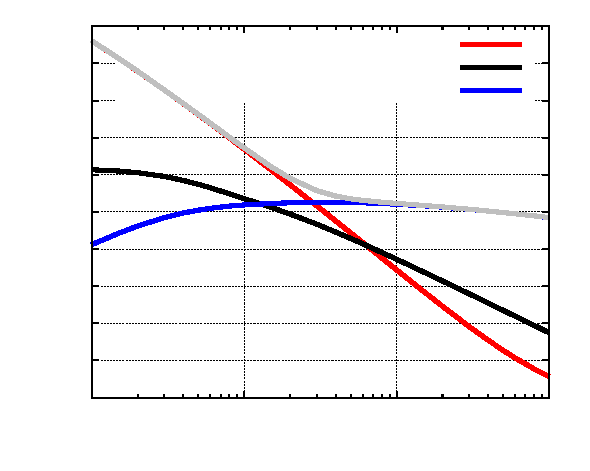
\includegraphics{AttenuationWater}}%
    \gplfronttext
  \end{picture}%
\endgroup

		\caption[Contributions to the X-ray attenuation coefficient of water.]{The different contributions to the attenuation of water at room temperature are depicted as a function of the photon energy \citep{henke_x-ray_1993} and the total attenuation is the summation of all the other contributions. The pair production in nuclear and electron field can be neglected at the displayed photon energies.}
		\label{fig:AttenuationWater}
\end{figure}

The other relevant contributions in the X-ray range are related to scattering processes. In an inelastic scattering event, the energy of the incident photon is partially transfered to a loosely bound electron resulting in a scattered photon with a longer wavelength, according to the Compton relation $\Delta\lambda = \sfrac{h}{m_e c}\left( 1 - \cos{2\theta} \right) $ \citep{als-nielsen_elements_2011}, where $2\theta$ is the scattering angle. The Compton scattering is incoherent and contributes generally less than the elastic scattering at energies below 10 keV, as observed in figure \ref{fig:AttenuationWater}. Besides, the coherent scattering signal is the summation of the constructive interferences of the electromagnetic wave, which produces a higher scattering intensity than the inelastic scattering. In fact, the elastic scattering of X-rays, typically coherent, is the main process used in material investigations and the physical principle behind SAXS.

\subsection{Elastic scattering}
\label{sec:ElasticScattering}

When the wavelength of the scattered wave is the same than that of the incident one, the proccess is named elastic scattering or coherent scattering and the resulting intensity is the absolute square of the sum of the scattering amplitudes. In the following sections, the elastic scattering theory will be presented for the classical case and for an ensemble of electrons.

\subsubsection{Thomson scattering}

\begin{figure}%[htbp]
\centering
\def\svgwidth{0.95\linewidth}
\input{Figures/FraunhoferScheme.pdf_tex}
\caption[Schematics of a scattering process and graphical definition of $\vect{q}$.]{Scheme of an scattering event by an object with a potential function $\phi(\vect{r'})$ at a distance $\abs{\vect{r}}=r$. A geometrical definition of the momentum transfer vector $\vect{q}$ is depicted on the right hand side, where $\vect{k}$ and $\vect{k_s}$ are the incident and scattered wavevector respectively.}
\label{fig:FraunhoferScheme}
\end{figure}

Classically, the elastic scattering of a photon by a free electron is described by the conservation of the photon energy, i.e. the wavenumber of the scattered wave is the same than the incident one ($\abs{\vect{k_s}}=\abs{\vect{k}}$). Consequently for unpolarized incident radiation, the intensity of the scattered wave at a distance $r$ and with a scattering angle $2\theta$ is defined by \citep{warren_x-ray_1969}:

\begin{equation}
        I_{\text{scat}}\left( r,\theta \right)= I_0 \left( \frac{r_e}{r} \right) ^2 \left( \frac{1+\cos^2{2\theta}}{2} \right)
\end{equation}

where $r_e= \sfrac{e^2}{4\pi\epsilon_0 m_e c^2}=2.82\cdot10^{-15}$ m is the Thomson or classical electron radius. A relevant quantity in scattering processes is the differential scattering cross-section $\sfrac{d\sigma}{d\Omega}$, which is directly proportional to the scattering intensity $I_{\text{scat}}$. It is defined as the the number of scattered photons per time and per solid angle over the incident intensity per time and per area \citep{als-nielsen_elements_2011}:

\begin{equation}
        \label{eq:thomson_cross_section}
        \frac{d\sigma}{d\Omega}= \frac{I_{\text{scat}} \cdot \left(r^2 \Delta \Omega \right)}{I_0\Delta \Omega}=r_e^2\left( \frac{1+\cos^2{2\theta}}{2} \right)
\end{equation}

where $r^2 \Delta \Omega$ is the detector surface in the plane of the impact parameter. The total Thomson scattering cross-section is $\sigma = \sfrac{8\pi r_0^2}{3} = 0.665\cdot10^{-24}$ cm$^2$ and similarly to $\sfrac{d\sigma}{d\Omega}$ is proportional to $r_e^2$ and independent from the photon energy if the photon wavelength is distant of an X-ray absorption edge.

\subsubsection{Scattering by an ensemble of electrons}

The scattering of a photon by an ensemble of weakly bound electrons can be studied by considering the interaction of particles with a three-dimensional weak potential $V(\vect{r})=V_0 \cdot \phi(\vect{r})$, where $V_0$ is the strength of the potential and $\phi(\vect{r})$ is the so-called \emph{potential function}. The resulting wave can be expressed as a linear combination of the incident plane wave (see equation \ref{eq:IncidentWave}) and the scattered spherical wave at the position $\vect{r}$:

\begin{equation}
       \Psi\left( \vect{r} \right)= \Psi_0\left( \vect{r} \right) +  \Psi_{\text{scat}}\left( \vect{r} \right)
\end{equation}

Inserting this expression at the time-independent Schrödinger equation and considering the scattering wave as a perturbation produced by the scattering potential function $\phi(\vect{r})$ \citep{cowley_diffraction_1995}, it can be derived that

\begin{equation}
       \Psi_{\text{scat}}\left( \vect{r} \right)=C \int \frac{e^{ i k\abs{\vect{r}-\vect{r}'} } } {\abs{\vect{r}-\vect{r}'}} \phi(\vect{r}')   \Psi\left( \vect{r}' \right) d\vect{r}'^3
\end{equation}

where $C$ is the so-called \emph{scattering length}. If the detection position $\vect{r}$ is at distance much larger than the scattering object size, as outlined in figure \ref{fig:FraunhoferScheme}, the Fraunhofer approximation applies and $\abs{\vect{r}-\vect{r'}} \simeq r$ \citep{feigin_structure_1987}, resulting in

\begin{equation}
       \Psi_{\text{scat}}\left( \vect{r} \right)=C \frac{e^{i k r}}{r} \int e^{ -i \vect{k}\vect{r}' }  \phi(\vect{r}')   \Psi\left( \vect{r}' \right) d\vect{r}'^3
\end{equation}

Assuming that there are no multiple scattering events due to the low concentration of scatterers and that the interaction potential is weak, the first Born approximation can be employed ($ \Psi\left( \vect{r} \right) \simeq \Psi_0\left( \vect{r} \right)$) \citep{cowley_diffraction_1995}, leading to

\begin{equation}
       \Psi_{\text{scat}}\left( \vect{r} \right)=C A_0 \frac{e^{i k r}}{r} \int e^{ i \vect{q}\vect{r}' }  \phi(\vect{r}')  d\vect{r}'^3
\end{equation}

where $\vect{q}=\vect{k_s} - \vect{k}$ is the momentum transfer vector and $\vect{k_s}$ the scattered wavevector. Analogously to equation \ref{eq:thomson_cross_section}, the differential scattering cross-section is:

\begin{equation}
        \label{eq:rayleigh_cross_section}
\frac{d\sigma}{d\Omega}= \frac{\abs{\Psi_{\text{scat}}}^2 \cdot \left(r^2 \Delta \Omega \right)}{\abs{\Psi_{0}}^2\Delta \Omega}=r_e^2 \abs{f(\vect{q})}^2 =r_e^2 \; I(\vect{q})
\end{equation}

where $f(\vect{q})=\int e^{ i \vect{q}\vect{r}' }  \phi(\vect{r}')  d\vect{r}'^3$ is the scattering amplitude, $I(\vect{q}) = \abs{f(\vect{q})}^2$ is the scattering intensity and the scattering length is the classical electron radius $r_e$. The scattering amplitude  $f(\vect{q})$ is simply the Fourier transform of the scattering potential function $\phi(\vect{r})$.

This type of scattering mechanism is named Rayleigh-Gans-Debye when the refractive index of the object $n_{\text{obj}}$ is close to unity and the condition $\sfrac{2\pi}{\lambda} \cdot D \cdot  \abs{n_{\text{med}} - n_{\text{obj}}} \ll 1$ is fulfilled, being $D$ the size of the object and $n_{\text{med}}$ the refractive index of the suspending medium. For X-ray photons with wavelenghts $\lambda$ around 0.1 nm and nanoscaled objects, this approximation can be applied and it can be safely assumed that the same electromagnetic wave impinges each part of the object \citep{hulst_light_1957, barber_rayleigh-gans-debye_1978}. In the case of optical radiation scattered by colloids, the Mie scattering framework is used, while the Rayleigh scattering corresponds to light wavelengths much larger than the scattering object.

\subsubsection{Anomalous scattering}

In X-ray scattering experiments, the scattering centres are the electrons of the atom and the scattering potential function is the electron charge density about the nucleous, so $\phi(\vect{r})=\rho_e(\vect{r})$. The electron density is related to the atomic properties as introduced in equation \ref{eq:AttenuationMultiComponent} and therefore the scattering amplitude increases with the atomic number $Z$ as can be shown by calculating equation \ref{eq:rayleigh_cross_section} at the limit $\vect{q} \rightarrow 0$

\begin{equation}
        f(\vect{q} \rightarrow 0) = \int \rho_e(\vect{r}')  d\vect{r}'^3 = Z
\end{equation}

This is valid when the incident photon energy is much larger than the energy corresponding to a resonant excitation. When the X-ray energy is close to an absorption edge, the anomalous dispersion becomes relevant and the scattering amplitude depends on the energy of the X-ray by adding the anomalous corrections \citep{als-nielsen_elements_2011}:

\begin{equation}
        f(E) = f_0 + f'(E) + i f'' (E)
\end{equation}

where the imaginary part $f''$ is related to the attenuation coefficient $\mu$ by \citep{feigin_structure_1987}

\begin{equation}
        f'' (E) = \frac{A\rho}{2N_A r_e h c} E \mu(E)
\end{equation}

where $A$ is the atomic mass of the resonant atom and $\rho$ its mass density. The term $f'$ is related to the imaginary anomalous coefficient by the Kramers-Kronig relationship \citep{de_l._kronig_theory_1926,kramers_diffusion_1927}:

\begin{equation}
        f'(E) = \frac{2}{\pi} \int_0^{\infty} \frac{E'f''(E')dE'}{E^2 - E'^2}
\end{equation}

The values of the anomalous scattering amplitude $f(E)$ are usually calculated using the experimentally measured attenuation coefficient $\mu(E)$.

\section{Small-angle X-ray scattering}
\label{sec:SAXS_theory}

Small-angle X-ray scattering is a powerful technique that can elucidate the structural features of particles with sizes ranging from a few nanometres up to some hundreds of nanometres. By investigating the photons elastically scattered by the electron density distribution of the particle $\rho_e ( \vect{r} )$, the resulting patterns can be analysed employing equation \ref{eq:rayleigh_cross_section} to obtain information about the particle size, shape and composition. Two fundamental quantities in a SAXS experiment are the scattering intensity $I(\vect{q})$, proportional to $\sfrac{d\sigma}{d\Omega}$, and the scattering amplitude or \emph{form factor} $f(\vect{q})$. The latter is expressed for objects with spherical symmetry where $\rho_e(\vect{r})=\rho_e(r)$ by

\begin{equation}
        \label{eq:FormFactorSpherical}
        f(q)=4\pi \int_0^{\infty} r'^2 \rho_e(r')  \frac{\sin(qr')}{qr'}  dr'
\end{equation}

where the modulus of the momentum transfer vector is defined by $q=\abs{\vect{q}}=\abs{\vect{k_s} - \vect{k}}$. Considering that SAXS is an elastic scattering process ($\abs{\vect{k_s}}=\abs{\vect{k}}=\sfrac{2\pi}{\lambda}$), the momentum transfer is expressed as

\begin{equation}
q=\frac{4\pi }{\lambda}\sin\theta=\frac{4\pi E}{h c}\sin\theta ,
\end{equation}

where \(\theta\) is half of the scattering angle as depicted in figure \ref{fig:FraunhoferScheme}, \(h\) is the Planck constant and \(c\) is the speed of light.

The systems studied by SAXS in this work consist of particles suspended in a uniform medium, e.g. water or buffer, with a different electron density $\rho_{\text{medium}}$ than the studied particle. In fact, the measured scattering amplitude is the addition of the medium and the particle contributions. Therefore, the scattering of the studied object is expressed in terms of the \emph{contrast}, $\Delta \eta (\vect{r}) = \rho_e(\vect{r}) - \rho_{\text{medium}}$, the electron density difference between the particle and the embedded matrix or surrounding medium. This leads to a slight modification of equation \ref{eq:FormFactorSpherical}, where $\rho_e(r)$ can be substituted by the contrast $\Delta\eta(r)$ to distinguish the contribution of the investigated particle from that of the medium.

\subsection{Scattering by an ensemble of particles}

For diluted systems with low particle concentration, the wave scattered by a particle does not interfere coherently with the neighboring particles, hence the scattering intensity can be expressed as a sum of the scattering of the individual particles, i.e. the structure factor contribution can be neglected because $S(q)=1$ \citep{feigin_structure_1987}. Assuming this premise, the scattering intensity of an ensemble of randomly oriented spherically symmetric nanoparticles in a diluted suspension can be expressed as

\begin{equation}
\label{eq:intensity}
I(q)=N\int_{0}^{\infty} g(R)\left|f(q,R) \right|^2 dR,
\end{equation}

where \(N\) is the number of scatterers i.e particles, \(g(R)\) is their size distribution function and \(f(q,R)\) is the particle form factor, which depends on the radial structure of the particle as determined in equation \ref{eq:FormFactorSpherical}. Generally, the particles in suspension are not monodisperse and show a certain size distribution which is often related with their chemical preparation. For systems of relatively low size polydispersity, a gaussian size distribution is typically a good choice, which is expressed by:

\begin{equation}
        \label{eq:gauss_distribution}
       g_{\text{Gauss}}(R)=\frac{1}{\sigma_R \sqrt{2\pi}} e^{ - \frac{\left( R - \overline{R} \right)^2}{2\sigma_R^2} }
\end{equation}

where $\overline{R}$ is the mean radius of the particles and $\sigma_R$ is the standard deviation of the size distribution. For smaller particles or higher polydispersity degrees, a log-normal distribution is preferred, defined as

\begin{equation}
       g_{\text{LN}}(R)=\frac{1}{\sigma_R \sqrt{2\pi}} e^{ - \frac{\left( \ln(R) - \ln(\overline{R}) \right)^2}{2\sigma_R^2} }
\end{equation}

whose mean radius is given by $\overline{R} e^{\frac{\sigma_R^2}{2}}$ and the variance is $\overline{R}^2 e^{\sigma_R^2} (e^{\sigma_R^2} - 1)$. Other approaches to the size distribution of particles in solution are based in numerical techniques, like the Monte-Carlo approach to form-free particle size distributions \citep{pauw_improvements_2013}.

A useful parameter for comparative purposes between samples is the polydispersity degree $p_d$, which is defined as the full width at half maximum (FWHM) of the number-weighted particle size distribution divided by its average value. For a normal size distribution, the FWHM is simply $8\sqrt{2}$ times its standard deviation $\sigma_R$.

\subsection{The scattering curve}

The differential scattering cross-section $\sfrac{d\sigma}{d\Omega}$ is the fundamental measurand in a SAXS experiment, as described in section \ref{sec:ElasticScattering}. Nevertheless, some comparability challenges arise from this quantity as it depends on the sample volume $V$ used in the experiment. This can be solved by introducing the differential scattering cross-section per volume, historically given in cm$^{-1}$. The expression of this quantity is derived from equations \ref{eq:rayleigh_cross_section} and \ref{eq:intensity} and leads to:

\begin{equation}
\frac{d\Sigma}{d\Omega} (q) = \frac{\sfrac{d\sigma}{d\Omega}(q)}{V} = \frac{r_e^2 \; I(q)}{V} = r_e^2 \cdot \frac{N}{V} \cdot \int_0^{\infty} g(R) \abs{ f(q,R) }^2 dR
\end{equation}

where $\sfrac{N}{V}$ is the concentration of scatterers, i.e. particles.

%\begin{figure}
%	\centering
%        	\resizebox{.85\linewidth}{!}{% GNUPLOT: LaTeX picture with Postscript
\begingroup
  \makeatletter
  \providecommand\color[2][]{%
    \GenericError{(gnuplot) \space\space\space\@spaces}{%
      Package color not loaded in conjunction with
      terminal option `colourtext'%
    }{See the gnuplot documentation for explanation.%
    }{Either use 'blacktext' in gnuplot or load the package
      color.sty in LaTeX.}%
    \renewcommand\color[2][]{}%
  }%
  \providecommand\includegraphics[2][]{%
    \GenericError{(gnuplot) \space\space\space\@spaces}{%
      Package graphicx or graphics not loaded%
    }{See the gnuplot documentation for explanation.%
    }{The gnuplot epslatex terminal needs graphicx.sty or graphics.sty.}%
    \renewcommand\includegraphics[2][]{}%
  }%
  \providecommand\rotatebox[2]{#2}%
  \@ifundefined{ifGPcolor}{%
    \newif\ifGPcolor
    \GPcolortrue
  }{}%
  \@ifundefined{ifGPblacktext}{%
    \newif\ifGPblacktext
    \GPblacktextfalse
  }{}%
  % define a \g@addto@macro without @ in the name:
  \let\gplgaddtomacro\g@addto@macro
  % define empty templates for all commands taking text:
  \gdef\gplbacktext{}%
  \gdef\gplfronttext{}%
  \makeatother
  \ifGPblacktext
    % no textcolor at all
    \def\colorrgb#1{}%
    \def\colorgray#1{}%
  \else
    % gray or color?
    \ifGPcolor
      \def\colorrgb#1{\color[rgb]{#1}}%
      \def\colorgray#1{\color[gray]{#1}}%
      \expandafter\def\csname LTw\endcsname{\color{white}}%
      \expandafter\def\csname LTb\endcsname{\color{black}}%
      \expandafter\def\csname LTa\endcsname{\color{black}}%
      \expandafter\def\csname LT0\endcsname{\color[rgb]{1,0,0}}%
      \expandafter\def\csname LT1\endcsname{\color[rgb]{0,1,0}}%
      \expandafter\def\csname LT2\endcsname{\color[rgb]{0,0,1}}%
      \expandafter\def\csname LT3\endcsname{\color[rgb]{1,0,1}}%
      \expandafter\def\csname LT4\endcsname{\color[rgb]{0,1,1}}%
      \expandafter\def\csname LT5\endcsname{\color[rgb]{1,1,0}}%
      \expandafter\def\csname LT6\endcsname{\color[rgb]{0,0,0}}%
      \expandafter\def\csname LT7\endcsname{\color[rgb]{1,0.3,0}}%
      \expandafter\def\csname LT8\endcsname{\color[rgb]{0.5,0.5,0.5}}%
    \else
      % gray
      \def\colorrgb#1{\color{black}}%
      \def\colorgray#1{\color[gray]{#1}}%
      \expandafter\def\csname LTw\endcsname{\color{white}}%
      \expandafter\def\csname LTb\endcsname{\color{black}}%
      \expandafter\def\csname LTa\endcsname{\color{black}}%
      \expandafter\def\csname LT0\endcsname{\color{black}}%
      \expandafter\def\csname LT1\endcsname{\color{black}}%
      \expandafter\def\csname LT2\endcsname{\color{black}}%
      \expandafter\def\csname LT3\endcsname{\color{black}}%
      \expandafter\def\csname LT4\endcsname{\color{black}}%
      \expandafter\def\csname LT5\endcsname{\color{black}}%
      \expandafter\def\csname LT6\endcsname{\color{black}}%
      \expandafter\def\csname LT7\endcsname{\color{black}}%
      \expandafter\def\csname LT8\endcsname{\color{black}}%
    \fi
  \fi
    \setlength{\unitlength}{0.0500bp}%
    \ifx\gptboxheight\undefined%
      \newlength{\gptboxheight}%
      \newlength{\gptboxwidth}%
      \newsavebox{\gptboxtext}%
    \fi%
    \setlength{\fboxrule}{0.5pt}%
    \setlength{\fboxsep}{1pt}%
\begin{picture}(5668.00,4534.00)%
    \gplgaddtomacro\gplbacktext{%
    }%
    \gplgaddtomacro\gplfronttext{%
      \csname LTb\endcsname%
      \put(176,2486){\rotatebox{-270}{\makebox(0,0){\strut{}$\sfrac{d \Sigma}{d \Omega}$ / cm$^{-1}$}}}%
      \put(3108,154){\makebox(0,0){\strut{}$q$ / nm$^{-1}$}}%
      \csname LTb\endcsname%
      \put(814,704){\makebox(0,0)[r]{\strut{}$10^{-4}$}}%
      \csname LTb\endcsname%
      \put(814,1213){\makebox(0,0)[r]{\strut{}$10^{-3}$}}%
      \csname LTb\endcsname%
      \put(814,1723){\makebox(0,0)[r]{\strut{}$10^{-2}$}}%
      \csname LTb\endcsname%
      \put(814,2232){\makebox(0,0)[r]{\strut{}$10^{-1}$}}%
      \csname LTb\endcsname%
      \put(814,2741){\makebox(0,0)[r]{\strut{}$10^{0}$}}%
      \csname LTb\endcsname%
      \put(814,3250){\makebox(0,0)[r]{\strut{}$10^{1}$}}%
      \csname LTb\endcsname%
      \put(814,3760){\makebox(0,0)[r]{\strut{}$10^{2}$}}%
      \csname LTb\endcsname%
      \put(814,4269){\makebox(0,0)[r]{\strut{}$10^{3}$}}%
      \csname LTb\endcsname%
      \put(946,484){\makebox(0,0){\strut{}$0.01$}}%
      \csname LTb\endcsname%
      \put(3108,484){\makebox(0,0){\strut{}$0.1$}}%
      \csname LTb\endcsname%
      \put(5271,484){\makebox(0,0){\strut{}$1$}}%
      \put(1117,4066){\makebox(0,0)[l]{\strut{}Guinier region}}%
      \put(4521,4066){\makebox(0,0)[l]{\strut{}Porod}}%
      \put(4521,3846){\makebox(0,0)[l]{\strut{}region}}%
      \put(2911,4066){\makebox(0,0)[l]{\strut{}Fourier region}}%
    }%
    \gplbacktext
    \put(0,0){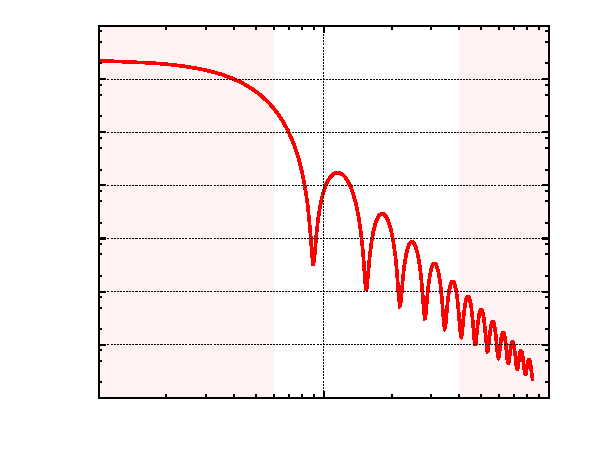
\includegraphics{ScatteringCurve50nm}}%
    \gplfronttext
  \end{picture}%
\endgroup
}
		%% GNUPLOT: LaTeX picture with Postscript
\begingroup
  \makeatletter
  \providecommand\color[2][]{%
    \GenericError{(gnuplot) \space\space\space\@spaces}{%
      Package color not loaded in conjunction with
      terminal option `colourtext'%
    }{See the gnuplot documentation for explanation.%
    }{Either use 'blacktext' in gnuplot or load the package
      color.sty in LaTeX.}%
    \renewcommand\color[2][]{}%
  }%
  \providecommand\includegraphics[2][]{%
    \GenericError{(gnuplot) \space\space\space\@spaces}{%
      Package graphicx or graphics not loaded%
    }{See the gnuplot documentation for explanation.%
    }{The gnuplot epslatex terminal needs graphicx.sty or graphics.sty.}%
    \renewcommand\includegraphics[2][]{}%
  }%
  \providecommand\rotatebox[2]{#2}%
  \@ifundefined{ifGPcolor}{%
    \newif\ifGPcolor
    \GPcolortrue
  }{}%
  \@ifundefined{ifGPblacktext}{%
    \newif\ifGPblacktext
    \GPblacktextfalse
  }{}%
  % define a \g@addto@macro without @ in the name:
  \let\gplgaddtomacro\g@addto@macro
  % define empty templates for all commands taking text:
  \gdef\gplbacktext{}%
  \gdef\gplfronttext{}%
  \makeatother
  \ifGPblacktext
    % no textcolor at all
    \def\colorrgb#1{}%
    \def\colorgray#1{}%
  \else
    % gray or color?
    \ifGPcolor
      \def\colorrgb#1{\color[rgb]{#1}}%
      \def\colorgray#1{\color[gray]{#1}}%
      \expandafter\def\csname LTw\endcsname{\color{white}}%
      \expandafter\def\csname LTb\endcsname{\color{black}}%
      \expandafter\def\csname LTa\endcsname{\color{black}}%
      \expandafter\def\csname LT0\endcsname{\color[rgb]{1,0,0}}%
      \expandafter\def\csname LT1\endcsname{\color[rgb]{0,1,0}}%
      \expandafter\def\csname LT2\endcsname{\color[rgb]{0,0,1}}%
      \expandafter\def\csname LT3\endcsname{\color[rgb]{1,0,1}}%
      \expandafter\def\csname LT4\endcsname{\color[rgb]{0,1,1}}%
      \expandafter\def\csname LT5\endcsname{\color[rgb]{1,1,0}}%
      \expandafter\def\csname LT6\endcsname{\color[rgb]{0,0,0}}%
      \expandafter\def\csname LT7\endcsname{\color[rgb]{1,0.3,0}}%
      \expandafter\def\csname LT8\endcsname{\color[rgb]{0.5,0.5,0.5}}%
    \else
      % gray
      \def\colorrgb#1{\color{black}}%
      \def\colorgray#1{\color[gray]{#1}}%
      \expandafter\def\csname LTw\endcsname{\color{white}}%
      \expandafter\def\csname LTb\endcsname{\color{black}}%
      \expandafter\def\csname LTa\endcsname{\color{black}}%
      \expandafter\def\csname LT0\endcsname{\color{black}}%
      \expandafter\def\csname LT1\endcsname{\color{black}}%
      \expandafter\def\csname LT2\endcsname{\color{black}}%
      \expandafter\def\csname LT3\endcsname{\color{black}}%
      \expandafter\def\csname LT4\endcsname{\color{black}}%
      \expandafter\def\csname LT5\endcsname{\color{black}}%
      \expandafter\def\csname LT6\endcsname{\color{black}}%
      \expandafter\def\csname LT7\endcsname{\color{black}}%
      \expandafter\def\csname LT8\endcsname{\color{black}}%
    \fi
  \fi
    \setlength{\unitlength}{0.0500bp}%
    \ifx\gptboxheight\undefined%
      \newlength{\gptboxheight}%
      \newlength{\gptboxwidth}%
      \newsavebox{\gptboxtext}%
    \fi%
    \setlength{\fboxrule}{0.5pt}%
    \setlength{\fboxsep}{1pt}%
\begin{picture}(5668.00,4534.00)%
    \gplgaddtomacro\gplbacktext{%
    }%
    \gplgaddtomacro\gplfronttext{%
      \csname LTb\endcsname%
      \put(176,2486){\rotatebox{-270}{\makebox(0,0){\strut{}$\sfrac{d \Sigma}{d \Omega}$ / cm$^{-1}$}}}%
      \put(3108,154){\makebox(0,0){\strut{}$q$ / nm$^{-1}$}}%
      \csname LTb\endcsname%
      \put(814,704){\makebox(0,0)[r]{\strut{}$10^{-4}$}}%
      \csname LTb\endcsname%
      \put(814,1213){\makebox(0,0)[r]{\strut{}$10^{-3}$}}%
      \csname LTb\endcsname%
      \put(814,1723){\makebox(0,0)[r]{\strut{}$10^{-2}$}}%
      \csname LTb\endcsname%
      \put(814,2232){\makebox(0,0)[r]{\strut{}$10^{-1}$}}%
      \csname LTb\endcsname%
      \put(814,2741){\makebox(0,0)[r]{\strut{}$10^{0}$}}%
      \csname LTb\endcsname%
      \put(814,3250){\makebox(0,0)[r]{\strut{}$10^{1}$}}%
      \csname LTb\endcsname%
      \put(814,3760){\makebox(0,0)[r]{\strut{}$10^{2}$}}%
      \csname LTb\endcsname%
      \put(814,4269){\makebox(0,0)[r]{\strut{}$10^{3}$}}%
      \csname LTb\endcsname%
      \put(946,484){\makebox(0,0){\strut{}$0.01$}}%
      \csname LTb\endcsname%
      \put(3108,484){\makebox(0,0){\strut{}$0.1$}}%
      \csname LTb\endcsname%
      \put(5271,484){\makebox(0,0){\strut{}$1$}}%
      \put(1117,4066){\makebox(0,0)[l]{\strut{}Guinier region}}%
      \put(4521,4066){\makebox(0,0)[l]{\strut{}Porod}}%
      \put(4521,3846){\makebox(0,0)[l]{\strut{}region}}%
      \put(2911,4066){\makebox(0,0)[l]{\strut{}Fourier region}}%
    }%
    \gplbacktext
    \put(0,0){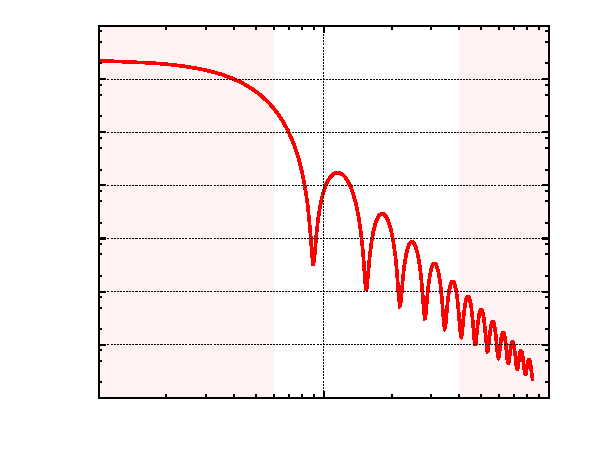
\includegraphics{ScatteringCurve50nm}}%
    \gplfronttext
  \end{picture}%
\endgroup

%		\caption[The scattering curve and its relevant regions.]{Simulated scattering curve of a nanoparticle ensemble with radius 50 nm and a polydispersity degree of 10 $\%$. The three different regions discussed in the text are highlighted in the figure as well.}
%		\label{fig:ScatteringCurve50nm}
%\end{figure}

\begin{figure*}%[htbp]
	\centering
		\subfloat[The scattering pattern]{\resizebox{0.35\linewidth}{!}{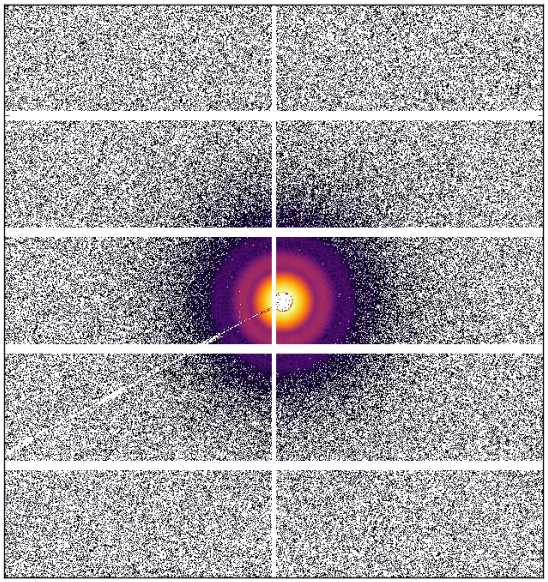
\includegraphics{Figures/Au100ScatteringPattern_edit2}}\label{fig:Au100ScatteringPattern}}
		\qquad
		\subfloat[The scattering curve and its relevant regions.]{\resizebox{0.5\linewidth}{!}{\figfont{12pt}% GNUPLOT: LaTeX picture with Postscript
\begingroup
  \makeatletter
  \providecommand\color[2][]{%
    \GenericError{(gnuplot) \space\space\space\@spaces}{%
      Package color not loaded in conjunction with
      terminal option `colourtext'%
    }{See the gnuplot documentation for explanation.%
    }{Either use 'blacktext' in gnuplot or load the package
      color.sty in LaTeX.}%
    \renewcommand\color[2][]{}%
  }%
  \providecommand\includegraphics[2][]{%
    \GenericError{(gnuplot) \space\space\space\@spaces}{%
      Package graphicx or graphics not loaded%
    }{See the gnuplot documentation for explanation.%
    }{The gnuplot epslatex terminal needs graphicx.sty or graphics.sty.}%
    \renewcommand\includegraphics[2][]{}%
  }%
  \providecommand\rotatebox[2]{#2}%
  \@ifundefined{ifGPcolor}{%
    \newif\ifGPcolor
    \GPcolortrue
  }{}%
  \@ifundefined{ifGPblacktext}{%
    \newif\ifGPblacktext
    \GPblacktextfalse
  }{}%
  % define a \g@addto@macro without @ in the name:
  \let\gplgaddtomacro\g@addto@macro
  % define empty templates for all commands taking text:
  \gdef\gplbacktext{}%
  \gdef\gplfronttext{}%
  \makeatother
  \ifGPblacktext
    % no textcolor at all
    \def\colorrgb#1{}%
    \def\colorgray#1{}%
  \else
    % gray or color?
    \ifGPcolor
      \def\colorrgb#1{\color[rgb]{#1}}%
      \def\colorgray#1{\color[gray]{#1}}%
      \expandafter\def\csname LTw\endcsname{\color{white}}%
      \expandafter\def\csname LTb\endcsname{\color{black}}%
      \expandafter\def\csname LTa\endcsname{\color{black}}%
      \expandafter\def\csname LT0\endcsname{\color[rgb]{1,0,0}}%
      \expandafter\def\csname LT1\endcsname{\color[rgb]{0,1,0}}%
      \expandafter\def\csname LT2\endcsname{\color[rgb]{0,0,1}}%
      \expandafter\def\csname LT3\endcsname{\color[rgb]{1,0,1}}%
      \expandafter\def\csname LT4\endcsname{\color[rgb]{0,1,1}}%
      \expandafter\def\csname LT5\endcsname{\color[rgb]{1,1,0}}%
      \expandafter\def\csname LT6\endcsname{\color[rgb]{0,0,0}}%
      \expandafter\def\csname LT7\endcsname{\color[rgb]{1,0.3,0}}%
      \expandafter\def\csname LT8\endcsname{\color[rgb]{0.5,0.5,0.5}}%
    \else
      % gray
      \def\colorrgb#1{\color{black}}%
      \def\colorgray#1{\color[gray]{#1}}%
      \expandafter\def\csname LTw\endcsname{\color{white}}%
      \expandafter\def\csname LTb\endcsname{\color{black}}%
      \expandafter\def\csname LTa\endcsname{\color{black}}%
      \expandafter\def\csname LT0\endcsname{\color{black}}%
      \expandafter\def\csname LT1\endcsname{\color{black}}%
      \expandafter\def\csname LT2\endcsname{\color{black}}%
      \expandafter\def\csname LT3\endcsname{\color{black}}%
      \expandafter\def\csname LT4\endcsname{\color{black}}%
      \expandafter\def\csname LT5\endcsname{\color{black}}%
      \expandafter\def\csname LT6\endcsname{\color{black}}%
      \expandafter\def\csname LT7\endcsname{\color{black}}%
      \expandafter\def\csname LT8\endcsname{\color{black}}%
    \fi
  \fi
    \setlength{\unitlength}{0.0500bp}%
    \ifx\gptboxheight\undefined%
      \newlength{\gptboxheight}%
      \newlength{\gptboxwidth}%
      \newsavebox{\gptboxtext}%
    \fi%
    \setlength{\fboxrule}{0.5pt}%
    \setlength{\fboxsep}{1pt}%
\begin{picture}(5668.00,4534.00)%
    \gplgaddtomacro\gplbacktext{%
    }%
    \gplgaddtomacro\gplfronttext{%
      \csname LTb\endcsname%
      \put(176,2486){\rotatebox{-270}{\makebox(0,0){\strut{}$\sfrac{d \Sigma}{d \Omega}$ / cm$^{-1}$}}}%
      \put(3108,154){\makebox(0,0){\strut{}$q$ / nm$^{-1}$}}%
      \csname LTb\endcsname%
      \put(814,704){\makebox(0,0)[r]{\strut{}$10^{-4}$}}%
      \csname LTb\endcsname%
      \put(814,1213){\makebox(0,0)[r]{\strut{}$10^{-3}$}}%
      \csname LTb\endcsname%
      \put(814,1723){\makebox(0,0)[r]{\strut{}$10^{-2}$}}%
      \csname LTb\endcsname%
      \put(814,2232){\makebox(0,0)[r]{\strut{}$10^{-1}$}}%
      \csname LTb\endcsname%
      \put(814,2741){\makebox(0,0)[r]{\strut{}$10^{0}$}}%
      \csname LTb\endcsname%
      \put(814,3250){\makebox(0,0)[r]{\strut{}$10^{1}$}}%
      \csname LTb\endcsname%
      \put(814,3760){\makebox(0,0)[r]{\strut{}$10^{2}$}}%
      \csname LTb\endcsname%
      \put(814,4269){\makebox(0,0)[r]{\strut{}$10^{3}$}}%
      \csname LTb\endcsname%
      \put(946,484){\makebox(0,0){\strut{}$0.01$}}%
      \csname LTb\endcsname%
      \put(3108,484){\makebox(0,0){\strut{}$0.1$}}%
      \csname LTb\endcsname%
      \put(5271,484){\makebox(0,0){\strut{}$1$}}%
      \put(1117,4066){\makebox(0,0)[l]{\strut{}Guinier region}}%
      \put(4521,4066){\makebox(0,0)[l]{\strut{}Porod}}%
      \put(4521,3846){\makebox(0,0)[l]{\strut{}region}}%
      \put(2911,4066){\makebox(0,0)[l]{\strut{}Fourier region}}%
    }%
    \gplbacktext
    \put(0,0){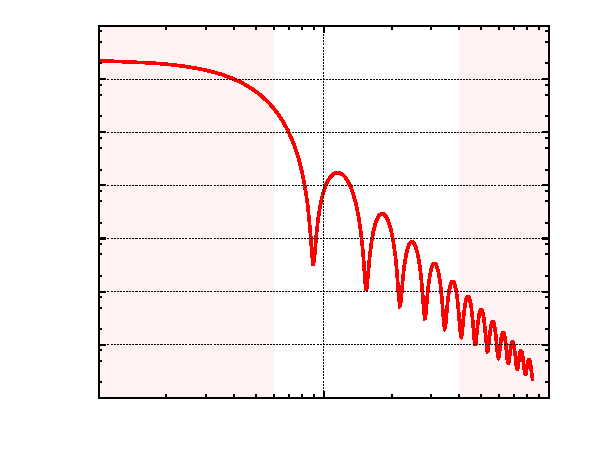
\includegraphics{ScatteringCurve50nm}}%
    \gplfronttext
  \end{picture}%
\endgroup
}\label{fig:ScatteringCurve50nm}}
\caption[The scattering curve and its relevant regions.]{a) Radially symmetric scattering pattern of a nanoparticle ensemble in suspension with radius 50 nm and a polydispersity degree of 25 $\%$. b) The scattering curve is the azimuthal integration of the 2D image. The three different regions of the scattering curve discussed in the text are highlighted in the figure as well.}
\end{figure*}

For isotropically scattering samples, the scattering patterns consist of concentric rings, as shown in figure \ref{fig:Au100ScatteringPattern}. By azimuthally averaging the scattering pattern, the data is reduced from 2D images to 1D scattering curves. The scattering curve is the typical form to present the experimental data, which displays the differential scattering cross-section per volume $\sfrac{d\Sigma}{d\Omega}$ versus the momentum transfer $q$ in a log–log graph as depicted in figure \ref{fig:ScatteringCurve50nm} for an ensemble of spherical particles with radius 50 nm and polydispersity degree 25 $\%$. Three different regions can be distinguished in a scattering curve \citep{schnablegger_practical_2006}:

\begin{itemize}
        \item The \textbf{Guinier region} comprises the low-$q$ region where $qD<1.3$ \citep{feigin_structure_1987}, being $D$ the characteristic length of the investigated object. This region provides principally information about the size of the particle.
        \item The high-$q$ region is called the \textbf{Porod region}, where information about the surface-to-volume ratio of the particles can be derived. For a smooth particle surface, the scattering intensity decays as $q^{-4}$, while for rough or fractal surfaces the slope is a function of $q^{-b}$ with $2<b<4$ \citep{glatter_small_1982}.
        \item For sufficiently monodisperse particle suspensions, the \textbf{Fourier region} or middle-$q$ region of the scattering curve shows pronounced minima that characterize the particle structure, size and shape.

\end{itemize}

\subsection{Modelling of the scattering intensity: Form factors}

Besides the information obtained about the size distribution of the particle ensemble, the scattering intensity $I(q)$ provides information about the shape and composition of the particles, accessible by modelling the form factor. In the simple case of a solid sphere with uniform density $\rho_0$, the radial electron density profile is described by $\rho_e(r>R)=0$ and $\rho_e(r<R)=\rho_0$, whilst the integral of expression \ref{eq:FormFactorSpherical} is limited only to the radius of the particle $R$. The form factor of a homogeneous solid sphere is 

\begin{equation}
        \label{eq:ff_sphere}
       f_{\text{sph}}(q,R)=\frac{4}{3}\pi R^3 \left( \rho_0 - \rho_{\text{medium}} \right) \left( 3\frac{\sin(qR)-qR\cos(qR)}{\left( qR \right)^3} \right) = \Delta \eta \cdot F_{\text{sph}}(q,R)
\end{equation}

where $\Delta \eta = \rho_0 - \rho_{\text{medium}}$ is the contrast and $ F_{\text{sph}}(q,R)$ is defined for convenience. When the shape of the particle deviates from a sphere, the assumptions made in equation \ref{eq:FormFactorSpherical} are not applicable and the scattering intensity must be integrated over all available angles numerically. For a homogeneous ellipsoid of revolution with two equal semi-axes of length $R$ and a semi-principal axis of length $\nu R $, the square of the form factor is expressed as:

\begin{equation}
        \label{eq:ff_ellipsoid}
       \abs{ f_{\text{ellip}}(q,R) }^2 = \Delta \eta^2 \int_0^1 \abs{F_{\text{sph}}\left( q,R \sqrt{u^2\left( \nu^2 -1 \right) + 1} \right)}^2 du
\end{equation}

where $\nu$ is the ellipticity, $u = \cos{\alpha}$ and $\alpha \in \left[  0, \sfrac{\pi}{2} \right]$. If $\nu > 1$, the expression defines a prolate spheroid, whilst $\nu < 1$ defines an oblate spheroid.

Frequently, nanoparticles show an internal heterogeneity, leading to an inner electron density distribution. If the components are radially distinguishable, the form factor corresponding to a morphology defined by sharp interfaces between the radial symmetric components of the particle with radius \(R_i\) is

\begin{equation}
\label{eq:multicore-shell}
f\left(q,R \right)= \Delta \eta F_{\text{sph}}(q,R)+\sum_{i=1}^{n-1} \Delta\rho_i \left( F_{\text{sph}}(q,R_{i+1})-F_{\text{sph}}(q,R_{i}) \right) ,
\end{equation}

where \(R\) is the external radius of the particle and \( n \) is the number of concentric shells. The excess of electron density of each component is $\Delta\rho_i = \rho_i - \rho_{\text{core}}$ and the contrast is defined in this case as $\Delta \eta = \rho_{\text{core}} - \rho_{\text{medium}}$ in order to isolate the electron density of the surrounding medium in one term.

The simplest case of expression \ref{eq:multicore-shell} arises for core-shell particles in suspension. This model represents a radially symmetric particle with a sharp interface between the outer shell and the inner core. The form factor is described by

\begin{equation}
        \label{eq:ff_cs}
	f_{\text{CS}}(q,R)=  \Delta\eta F_{\text{sph}}(q,R) +  \Delta\rho\left( F_{\text{sph}}(q,R)-F_{\text{sph}}(q,R_{\text{core}}) \right) ,
\end{equation}

where \(R \) and \(R_{\text{core}} \)  are the outer shell and inner core radii respectively, the excess of electron density is \(\Delta\rho=\rho_{\text{shell}}-\rho_{\text{core}}\) and the contrast is expressed as \(\Delta\eta=\rho_{\text{core}}-\rho_{\text{solv}}\), where $\rho_{\text{solv}}$ is the electron density of the suspending medium.

Depending on the synthesis of the particles, the interface between the different phases might show a linear electron density gradient between the particle's components. Analogously to expression \ref{eq:multicore-shell}, the form factor of a multicomponent spherical particle with a linear gradient interface is

\begin{equation}
f\left(q,R \right) = \sum_{i=0}^{n-1}\left[m_i \left( F_{\text{lin}}(q,R_{i+1})-F_{\text{lin}}(q,R_{i}) \right) +b_i \left( F_{\text{sph}}(q,R_{i+1})-F_{\text{sph}}(q,R_{i}) \right) \right]
\end{equation}
where $m_i=\sfrac{\left( \rho_{i+1}-\rho_{i} \right)}{\left( R_{i+1}-R_{i} \right)}$ and $b_i=\left( \rho_i-\rho_{\text{solv}} \right)-R_im_i$ and the linear form factor is defined by
\begin{equation}
F_{\text{lin}}(q,R) = 4\pi\frac{ \left( 2qR\sin(qR)+2\cos(qR)-(qR)^2\cos(qR) \right)}{q^4}
\end{equation}

The presented form factors are the models used in this work to analyse the experimental SAXS data of nanoparticles in suspension which will be discussed in chapters \ref{chap:density_gradient_SAXS}, \ref{chap:simultaneous_size_density} and \ref{chap:bio_applications}.

\section{Contrast variation}
\label{sec:contrast_variation_theory}

In the contrast variation method, the electron density of the particle or the surrounding medium is systematically altered in order to obtain independent scattering curves with different contrasts $\Delta \eta (r)$. This technique is useful to characterize the different components of heterogeneous particles, due to the complementary data that can be collected at each contrast. The work presented in this thesis is focused in the \emph{solvent contrast variation} method, where only the electron density of the suspending medium is varied.

\begin{figure*}%[htbp]
	\centering
		\subfloat[Core-shell particle in solvent]{\resizebox{0.44\linewidth}{!}{\fontsize{25pt}{25pt}\selectfont\input{Figures/ContrastScheme.pdf_tex}}\label{fig:ContrastScheme}}
		\qquad
		\subfloat[Contrast matching of the shell]{\resizebox{0.44\linewidth}{!}{\fontsize{25pt}{25pt}\selectfont\input{Figures/MatchPointScheme.pdf_tex}}\label{fig:MatchPointScheme}}
	\caption[Solvent contrast variation experiment and contrast matching scheme.]{Variation of the solvent electron density represented by the electron density profile of a spherical core-shell particle: a) The contrast of both core and shell components is high ($\Delta\eta_{\text{core}} > \Delta\eta_{\text{shell}} > 0$), while in figure b) the solvent electron density is increased to match the shell's ($\Delta\eta_{\text{shell}} = 0$). In this case, the only contribution to the scattering intensity will arise from the core.}
\end{figure*}


By means of the solvent contrast variation approach, the electron density of a single phase of the investigated particle can be matched (i.e. \emph{match point}), resulting in a increased scattering amplitude of the other components of the object, as depicted in figures \ref{fig:ContrastScheme} and \ref{fig:MatchPointScheme}. This effect enables a much more detailed study of the different contributions of the particle's components to the scattering intensity, which can be isolated by choosing the solvent electron density appropriately. In the following paragraphs, the theoretical framework required to interpret a SAXS contrast variation experiment will be presented, focusing mainly on the effects produced by the variation of the solvent electron density $\rho_{\text{solv}}$.

 
\subsection{Isoscattering point}
\label{sec:isopoint_theory}
One of the best known features appearing in a contrast variation experiment with heterogeneous nanoparticles is the existence of \emph{isoscattering points}, first formulated by \cite{kawaguchi_x-ray_1983-1}. At these specific \( q\)-values, the scattering intensity is independent of the adjusted solvent contrast, i.e. all scattering curves intersect in the isoscattering points regardless of the contrast. The isoscattering points \(q^{\star}\) are particularly interesting because they emerge for any spherical particle with an inner structure and a sufficiently narrow size distribution. From the contrast-depending part of equation \eqref{eq:multicore-shell}, a model-free expression can be derived which relates the position of the isoscattering points \(q^{\star}_i\) with the external radius of the particle \( R \), independent of its radial structure \citep{kawaguchi_x-ray_1983-1,kawaguchi_isoscattering_1992}:

\begin{equation}
        \label{eq:isoscattering}
        \tan(q^{\star}_iR)=q^{\star}_iR
\end{equation}

The solutions for this equation fulfill $q^{\star} R =4.493, 7.725, 10.904, ...$, where the positions of the isoscattering points correspond to the minima positions of the scattering intensity of a compact spherical particle with radius \( R \). This expression relates in a simple way the position of $q^{\star}$ to the size of the particle inaccessible to the suspending medium and, thus, a good method to determine the diameter of the colloid.

Although this expression is derived for the monodisperse case, it can still be applied up to a moderate degree of polydispersity, if care is taken regarding the shift of the minima position due to polydispersity \citep{beurten_polydispersity_1981}. For size distributions with \( p_d\) larger than \( \approx 30\,\% \), the isoscattering point is not well defined and the intersection point of the curves is smeared out, showing a diffuseness in the isoscattering point position \citep{kawaguchi_isoscattering_1992}. The effect of polydispersity in the isoscattering point is illustrated by simulating a 100 nm core-shell particle for the ideal case of a monodisperse ensemble (figure \ref{fig:IsopointSimulationIdeal}) and with a degree of polydispersity of 30 $\%$ (figure \ref{fig:IsopointSimulationPolydisperse}). The shift of the isoscatterig point position to smaller $q$-values and the diffuseness of the intersection point due to the high $p_d$ are clearly evident in the inset of figure \ref{fig:IsopointSimulationPolydisperse}.

Similarly, any deviation from the spherical shape produces a diffuseness in the $q^{\star}$ position. Unfortunately, this effect cannot be distinguished from the smearing produced by the size polydispersity and the investigation of the particle shape needs to be performed by other means.

\begin{figure*}%[htbp]
	\centering
		\subfloat[Monodisperse nanoparticles]{\resizebox{0.45\linewidth}{!}{\figfont{12pt}% GNUPLOT: LaTeX picture with Postscript
\begingroup
  \makeatletter
  \providecommand\color[2][]{%
    \GenericError{(gnuplot) \space\space\space\@spaces}{%
      Package color not loaded in conjunction with
      terminal option `colourtext'%
    }{See the gnuplot documentation for explanation.%
    }{Either use 'blacktext' in gnuplot or load the package
      color.sty in LaTeX.}%
    \renewcommand\color[2][]{}%
  }%
  \providecommand\includegraphics[2][]{%
    \GenericError{(gnuplot) \space\space\space\@spaces}{%
      Package graphicx or graphics not loaded%
    }{See the gnuplot documentation for explanation.%
    }{The gnuplot epslatex terminal needs graphicx.sty or graphics.sty.}%
    \renewcommand\includegraphics[2][]{}%
  }%
  \providecommand\rotatebox[2]{#2}%
  \@ifundefined{ifGPcolor}{%
    \newif\ifGPcolor
    \GPcolortrue
  }{}%
  \@ifundefined{ifGPblacktext}{%
    \newif\ifGPblacktext
    \GPblacktextfalse
  }{}%
  % define a \g@addto@macro without @ in the name:
  \let\gplgaddtomacro\g@addto@macro
  % define empty templates for all commands taking text:
  \gdef\gplbacktext{}%
  \gdef\gplfronttext{}%
  \makeatother
  \ifGPblacktext
    % no textcolor at all
    \def\colorrgb#1{}%
    \def\colorgray#1{}%
  \else
    % gray or color?
    \ifGPcolor
      \def\colorrgb#1{\color[rgb]{#1}}%
      \def\colorgray#1{\color[gray]{#1}}%
      \expandafter\def\csname LTw\endcsname{\color{white}}%
      \expandafter\def\csname LTb\endcsname{\color{black}}%
      \expandafter\def\csname LTa\endcsname{\color{black}}%
      \expandafter\def\csname LT0\endcsname{\color[rgb]{1,0,0}}%
      \expandafter\def\csname LT1\endcsname{\color[rgb]{0,1,0}}%
      \expandafter\def\csname LT2\endcsname{\color[rgb]{0,0,1}}%
      \expandafter\def\csname LT3\endcsname{\color[rgb]{1,0,1}}%
      \expandafter\def\csname LT4\endcsname{\color[rgb]{0,1,1}}%
      \expandafter\def\csname LT5\endcsname{\color[rgb]{1,1,0}}%
      \expandafter\def\csname LT6\endcsname{\color[rgb]{0,0,0}}%
      \expandafter\def\csname LT7\endcsname{\color[rgb]{1,0.3,0}}%
      \expandafter\def\csname LT8\endcsname{\color[rgb]{0.5,0.5,0.5}}%
    \else
      % gray
      \def\colorrgb#1{\color{black}}%
      \def\colorgray#1{\color[gray]{#1}}%
      \expandafter\def\csname LTw\endcsname{\color{white}}%
      \expandafter\def\csname LTb\endcsname{\color{black}}%
      \expandafter\def\csname LTa\endcsname{\color{black}}%
      \expandafter\def\csname LT0\endcsname{\color{black}}%
      \expandafter\def\csname LT1\endcsname{\color{black}}%
      \expandafter\def\csname LT2\endcsname{\color{black}}%
      \expandafter\def\csname LT3\endcsname{\color{black}}%
      \expandafter\def\csname LT4\endcsname{\color{black}}%
      \expandafter\def\csname LT5\endcsname{\color{black}}%
      \expandafter\def\csname LT6\endcsname{\color{black}}%
      \expandafter\def\csname LT7\endcsname{\color{black}}%
      \expandafter\def\csname LT8\endcsname{\color{black}}%
    \fi
  \fi
  \setlength{\unitlength}{0.0500bp}%
  \begin{picture}(5668.00,4534.00)%
    \gplgaddtomacro\gplbacktext{%
      \csname LTb\endcsname%
      \put(748,851){\makebox(0,0)[r]{\strut{}$10^{1}$}}%
      \csname LTb\endcsname%
      \put(748,1339){\makebox(0,0)[r]{\strut{}$10^{2}$}}%
      \csname LTb\endcsname%
      \put(748,1828){\makebox(0,0)[r]{\strut{}$10^{3}$}}%
      \csname LTb\endcsname%
      \put(748,2316){\makebox(0,0)[r]{\strut{}$10^{4}$}}%
      \csname LTb\endcsname%
      \put(748,2804){\makebox(0,0)[r]{\strut{}$10^{5}$}}%
      \csname LTb\endcsname%
      \put(748,3292){\makebox(0,0)[r]{\strut{}$10^{6}$}}%
      \csname LTb\endcsname%
      \put(748,3781){\makebox(0,0)[r]{\strut{}$10^{7}$}}%
      \csname LTb\endcsname%
      \put(748,4269){\makebox(0,0)[r]{\strut{}$10^{8}$}}%
      \csname LTb\endcsname%
      \put(1365,484){\makebox(0,0){\strut{} 0.02}}%
      \csname LTb\endcsname%
      \put(2235,484){\makebox(0,0){\strut{} 0.05}}%
      \csname LTb\endcsname%
      \put(2894,484){\makebox(0,0){\strut{} 0.1}}%
      \csname LTb\endcsname%
      \put(3552,484){\makebox(0,0){\strut{} 0.2}}%
      \csname LTb\endcsname%
      \put(4422,484){\makebox(0,0){\strut{} 0.5}}%
      \put(176,2486){\rotatebox{-270}{\makebox(0,0){\strut{}Scattering Intensity / a.u.}}}%
      \put(2651,154){\makebox(0,0){\strut{}$q$ / nm$^{-1}$}}%
    }%
    \gplgaddtomacro\gplfronttext{%
      \csname LTb\endcsname%
      \put(4853,704){\makebox(0,0)[l]{\strut{}\smaller -100}}%
      \put(4853,1149){\makebox(0,0)[l]{\strut{}\smaller -80}}%
      \put(4853,1595){\makebox(0,0)[l]{\strut{}\smaller -60}}%
      \put(4853,2040){\makebox(0,0)[l]{\strut{}\smaller -40}}%
      \put(4853,2486){\makebox(0,0)[l]{\strut{}\smaller -20}}%
      \put(4853,2932){\makebox(0,0)[l]{\strut{}\smaller 0}}%
      \put(4853,3377){\makebox(0,0)[l]{\strut{}\smaller 20}}%
      \put(4853,3823){\makebox(0,0)[l]{\strut{}\smaller 40}}%
      \put(4853,4269){\makebox(0,0)[l]{\strut{}\smaller 60}}%
      \put(5283,2486){\rotatebox{-90}{\makebox(0,0){\strut{}\smaller $\Delta \eta$ / nm$^{-3}$}}}%
    }%
    \gplgaddtomacro\gplbacktext{%
      \csname LTb\endcsname%
      \put(3334,3131){\makebox(0,0){\strut{}\smaller 0.08}}%
      \csname LTb\endcsname%
      \put(3817,3131){\makebox(0,0){\strut{}\smaller 0.09}}%
      \csname LTb\endcsname%
      \put(4250,3131){\makebox(0,0){\strut{}\smaller 0.1}}%
    }%
    \gplgaddtomacro\gplfronttext{%
    }%
    \gplbacktext
    \put(0,0){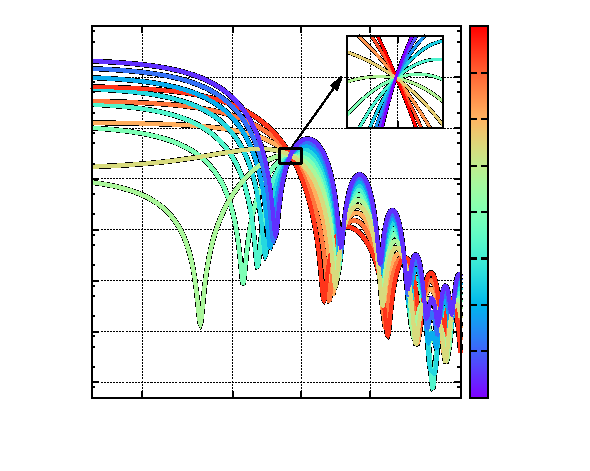
\includegraphics{IsopointSimulationIdeal}}%
    \gplfronttext
  \end{picture}%
\endgroup
}\label{fig:IsopointSimulationIdeal}}
		\qquad
		\subfloat[Polydisperse ensemble: $p_d=30\;\%$]{\resizebox{0.45\linewidth}{!}{\figfont{12pt}% GNUPLOT: LaTeX picture with Postscript
\begingroup
  \makeatletter
  \providecommand\color[2][]{%
    \GenericError{(gnuplot) \space\space\space\@spaces}{%
      Package color not loaded in conjunction with
      terminal option `colourtext'%
    }{See the gnuplot documentation for explanation.%
    }{Either use 'blacktext' in gnuplot or load the package
      color.sty in LaTeX.}%
    \renewcommand\color[2][]{}%
  }%
  \providecommand\includegraphics[2][]{%
    \GenericError{(gnuplot) \space\space\space\@spaces}{%
      Package graphicx or graphics not loaded%
    }{See the gnuplot documentation for explanation.%
    }{The gnuplot epslatex terminal needs graphicx.sty or graphics.sty.}%
    \renewcommand\includegraphics[2][]{}%
  }%
  \providecommand\rotatebox[2]{#2}%
  \@ifundefined{ifGPcolor}{%
    \newif\ifGPcolor
    \GPcolortrue
  }{}%
  \@ifundefined{ifGPblacktext}{%
    \newif\ifGPblacktext
    \GPblacktextfalse
  }{}%
  % define a \g@addto@macro without @ in the name:
  \let\gplgaddtomacro\g@addto@macro
  % define empty templates for all commands taking text:
  \gdef\gplbacktext{}%
  \gdef\gplfronttext{}%
  \makeatother
  \ifGPblacktext
    % no textcolor at all
    \def\colorrgb#1{}%
    \def\colorgray#1{}%
  \else
    % gray or color?
    \ifGPcolor
      \def\colorrgb#1{\color[rgb]{#1}}%
      \def\colorgray#1{\color[gray]{#1}}%
      \expandafter\def\csname LTw\endcsname{\color{white}}%
      \expandafter\def\csname LTb\endcsname{\color{black}}%
      \expandafter\def\csname LTa\endcsname{\color{black}}%
      \expandafter\def\csname LT0\endcsname{\color[rgb]{1,0,0}}%
      \expandafter\def\csname LT1\endcsname{\color[rgb]{0,1,0}}%
      \expandafter\def\csname LT2\endcsname{\color[rgb]{0,0,1}}%
      \expandafter\def\csname LT3\endcsname{\color[rgb]{1,0,1}}%
      \expandafter\def\csname LT4\endcsname{\color[rgb]{0,1,1}}%
      \expandafter\def\csname LT5\endcsname{\color[rgb]{1,1,0}}%
      \expandafter\def\csname LT6\endcsname{\color[rgb]{0,0,0}}%
      \expandafter\def\csname LT7\endcsname{\color[rgb]{1,0.3,0}}%
      \expandafter\def\csname LT8\endcsname{\color[rgb]{0.5,0.5,0.5}}%
    \else
      % gray
      \def\colorrgb#1{\color{black}}%
      \def\colorgray#1{\color[gray]{#1}}%
      \expandafter\def\csname LTw\endcsname{\color{white}}%
      \expandafter\def\csname LTb\endcsname{\color{black}}%
      \expandafter\def\csname LTa\endcsname{\color{black}}%
      \expandafter\def\csname LT0\endcsname{\color{black}}%
      \expandafter\def\csname LT1\endcsname{\color{black}}%
      \expandafter\def\csname LT2\endcsname{\color{black}}%
      \expandafter\def\csname LT3\endcsname{\color{black}}%
      \expandafter\def\csname LT4\endcsname{\color{black}}%
      \expandafter\def\csname LT5\endcsname{\color{black}}%
      \expandafter\def\csname LT6\endcsname{\color{black}}%
      \expandafter\def\csname LT7\endcsname{\color{black}}%
      \expandafter\def\csname LT8\endcsname{\color{black}}%
    \fi
  \fi
  \setlength{\unitlength}{0.0500bp}%
  \begin{picture}(5668.00,4534.00)%
    \gplgaddtomacro\gplbacktext{%
      \csname LTb\endcsname%
      \put(748,704){\makebox(0,0)[r]{\strut{}$10^{2}$}}%
      \csname LTb\endcsname%
      \put(748,1355){\makebox(0,0)[r]{\strut{}$10^{3}$}}%
      \csname LTb\endcsname%
      \put(748,2006){\makebox(0,0)[r]{\strut{}$10^{4}$}}%
      \csname LTb\endcsname%
      \put(748,2657){\makebox(0,0)[r]{\strut{}$10^{5}$}}%
      \csname LTb\endcsname%
      \put(748,3308){\makebox(0,0)[r]{\strut{}$10^{6}$}}%
      \csname LTb\endcsname%
      \put(748,3958){\makebox(0,0)[r]{\strut{}$10^{7}$}}%
      \csname LTb\endcsname%
      \put(1365,484){\makebox(0,0){\strut{} 0.02}}%
      \csname LTb\endcsname%
      \put(2235,484){\makebox(0,0){\strut{} 0.05}}%
      \csname LTb\endcsname%
      \put(2894,484){\makebox(0,0){\strut{} 0.1}}%
      \csname LTb\endcsname%
      \put(3552,484){\makebox(0,0){\strut{} 0.2}}%
      \csname LTb\endcsname%
      \put(4422,484){\makebox(0,0){\strut{} 0.5}}%
      \put(176,2486){\rotatebox{-270}{\makebox(0,0){\strut{}Scattering Intensity / a.u.}}}%
      \put(2651,154){\makebox(0,0){\strut{}$q$ / nm$^{-1}$}}%
    }%
    \gplgaddtomacro\gplfronttext{%
      \csname LTb\endcsname%
      \put(4853,704){\makebox(0,0)[l]{\strut{}\smaller -100}}%
      \put(4853,1149){\makebox(0,0)[l]{\strut{}\smaller -80}}%
      \put(4853,1595){\makebox(0,0)[l]{\strut{}\smaller -60}}%
      \put(4853,2040){\makebox(0,0)[l]{\strut{}\smaller -40}}%
      \put(4853,2486){\makebox(0,0)[l]{\strut{}\smaller -20}}%
      \put(4853,2932){\makebox(0,0)[l]{\strut{}\smaller 0}}%
      \put(4853,3377){\makebox(0,0)[l]{\strut{}\smaller 20}}%
      \put(4853,3823){\makebox(0,0)[l]{\strut{}\smaller 40}}%
      \put(4853,4269){\makebox(0,0)[l]{\strut{}\smaller 60}}%
      \put(5283,2486){\rotatebox{-90}{\makebox(0,0){\strut{}\smaller $\Delta \eta$ / nm$^{-3}$}}}%
    }%
    \gplgaddtomacro\gplbacktext{%
      \csname LTb\endcsname%
      \put(3609,3131){\makebox(0,0){\strut{}\smaller 0.08}}%
      \csname LTb\endcsname%
      \put(4110,3131){\makebox(0,0){\strut{}\smaller 0.09}}%
    }%
    \gplgaddtomacro\gplfronttext{%
    }%
    \gplbacktext
    \put(0,0){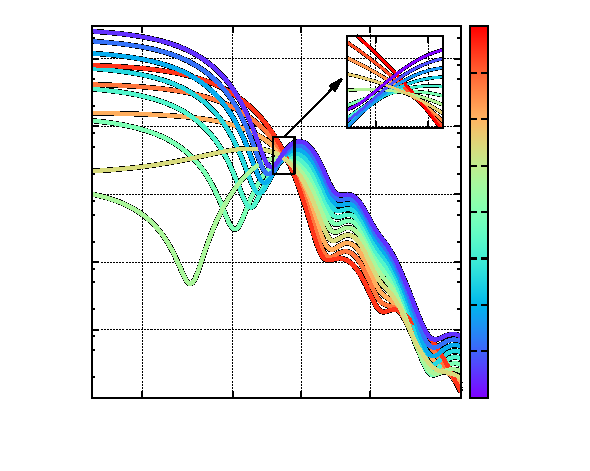
\includegraphics{IsopointSimulationPolydisperse}}%
    \gplfronttext
  \end{picture}%
\endgroup
}\label{fig:IsopointSimulationPolydisperse}}
	\caption[Isoscattering points and particle polydispersity.]{A isoscattering point is the $q$-value where all the scattering curves measured at different contrasts $\Delta \eta$ intersect. a) In the monodisperse case, the first isoscattering point is well-defined as depicted in the inset, while the inset of b) shows how the high polydispersity of the ensemble produces a diffuse isoscattering point and the intersection point is smeared out.}
\end{figure*}

\subsection{Basic functions approach}
\label{sec:basic_functions_theory}
When analysing contrast variation data, a widespread theoretical approach is based on the non-interacting model proposed by Stuhrmann $\&$ Kirste (\citeyear{stuhrmann_elimination_1965,stuhrmann_elimination_1967}) for monodisperse particles. The so-called \emph{basic functions} formulation differentiates, independently of the particle inner structure, the contributions which depend on the varying solvent density or contrast (\(\Delta\eta\)) and on the excess of electron density of each component of the particle.

Deriving from this approach, the scattering intensity can be expressed as the combination of contributions corresponding to different features of the particles:
\begin{equation}
\label{eq:intensity_contrast}
I(q)=I_c(q)+\Delta\eta I_{sc}(q)+(\Delta\eta)^2 I_{s}(q)
\end{equation}
The $I_c$ function contains the contributions from the density fluctuations inside the particle, the contribution $I_s$ is the so-called \emph{shape scattering function} and $I_{sc}$ is the cross-term function.

\subsubsection{Shape scattering function}
The $I_s(q)$ function corresponds to the scattering contributions from particles with homogeneous density and a size equivalent to the volume inaccessible to the solvent, typically the external size of the nanoparticle. By modelling the shape scattering function, the shape and size distribution of the particles can be determined independently of their inner structure. The functions $I_{sc}(q)$ and $I_{c}(q)$ are more rarely employed due to their complex interpretation. $I_{c}(q)$ contains the electron density deviations in the particle from the average electron density, while $I_{sc}(q)$ includes crossed contributions from both $I_{c}(q)$ and $I_{s}(q)$.

In a system measured at $N$ different solvent electron densities i.e. contrasts, the shape scattering function $I_s$ at each $q$-value can be calculated by solving the following matrix equation:

\begin{equation}
  \begin{pmatrix}
  I_1(q) \\
  \vdots \\
  I_N(q) \\
 \end{pmatrix}
  = 
 \begin{pmatrix}
  1 & \Delta \eta_1 &  \left( \Delta \eta_1 \right)^2 \\
  \vdots  & \vdots  & \vdots  \\
  1 & \Delta \eta_N &  \left( \Delta \eta_N \right)^2 
 \end{pmatrix}
 \begin{pmatrix}
  I_c(q) \\
  I_{sc}(q) \\
  I_s(q) \\
 \end{pmatrix}
\end{equation}

where $I_i (q)$ is the measured scattering intensity at each solvent electron density and $\Delta \eta _i$ is the contrast corresponding to each suspending medium density. A minimum of 3 independent scattering curves measured at different contrasts are required to solve this system of equations, while an accurate determination of the suspending medium electron density is also necessary for the calculation of the different $\Delta \eta _i$.

\subsubsection{Guinier approximation}
\label{sec:TheoryGuinier}

The radius of gyration of a particle about its centre of mass $R_g$ is defined as the second moment of the electron density distribution and can be calculated by 

\begin{equation}
        R_g^2 = \frac{\int \rho_e (r) r^2 dr}{\int \rho_e (r)  dr}
\end{equation}

The radius of gyration is systematically employed in small-angle scattering as an evaluation tool, due to its applicability to a large diversity of samples, e.g. proteins, colloids, suprastructures \citep{mertens_structural_2010,sim_salt_2012}. If the object is spherical, the gyration radius is directly related with its external radius by $R_g^2 = \sfrac{3}{5}R^2$.

In SAXS, $R_g$ can be calculated using the Guinier approximation \citep{guinier_diffraction_1939,guinier_small-angle_1955}, which assumes that the scattering intensity behaves in the limit of small \(q\) as

\begin{equation}
\label{eq:guinier}
I(q) \simeq I(0)\,\mbox{exp}\left(-\frac{R_g^2}{3}q^2\right),
\end{equation}

where \( I(0)\) is known as forward scattering or intensity at zero angle. Using the basic functions approach, the radius of gyration of a monodisperse, heterogeneous particle can be expressed as a function of the solvent electron density \( \rho_{\text{solv}} \) and the average electron density of the particle \( \rho_0 \) \citep{feigin_structure_1987}
\begin{equation}
R_g^2=R_{g,c}^{\,2}+\frac{\alpha}{\rho_0-\rho_{\text{solv}}}-\frac{\beta}{(\rho_0-\rho_{\text{solv}})^2},
\label{eq:gyration}
\end{equation}
where \(R_{g,c}\) is the radius of gyration of the particle shape corresponding to the volume inaccessible for the solvent \( V_c \), \( \alpha \) characterizes the distribution of different phases inside the particle and \( \beta>0 \) considers the eccentricity of the different scattering contributions \citep{stuhrmann_small-angle_2008}. Particle aggregation influences the scattering curves especially in the Guinier region and must be explicitly avoided.

\cite{avdeev_contrast_2007} proposed an extended version to equation \eqref{eq:gyration} for the case of a polydisperse particle ensemble by introducing the \emph{effective} values \( \tilde R^2_{g,c} \), \( \tilde \alpha \) and \( \tilde \beta \), which are the intensity-weighted averages of the corresponding parameters over the polydispersity. The observed average electron density is not affected by the polydispersity (\( \tilde\rho_0=\rho_0 \)) if the volume ratio between the different particle components is constant for all particles in the ensemble.

Assuming the premise of a constant average electron density for all the particles, the intensity at zero angle for a polydisperse system can be expressed as

\begin{equation}
\label{eq:I0}
I(0)\propto N \left( \rho_0-\rho_{\text{solv}} \right)^2 ,
\end{equation}

with a minimum of the parabolic function at \( \rho_{\text{solv}}=\rho_0 \). Therefore, by analysing the Guinier region of the scattering curves in a contrast variation experiment, the average electron density of the particle can be obtained without assuming an \emph{a priori} inner structure.

Using the models presented above, it is possible to obtain by independent means the external radius and the average electron density of the particles in suspension.
